\documentclass[12pt]{article}
\usepackage[utf8]{inputenc}
\usepackage[english]{babel}
\usepackage{geometry}
\usepackage{listings} % for code snippets
\usepackage{xcolor}
\usepackage{graphicx}
\usepackage{titlesec}

% page setup and spacing
\geometry{a4paper, margin=0.75in}
\setlength{\parindent}{1em}
\setlength{\parskip}{1em}
\renewcommand{\baselinestretch}{1.0}

% colors for code snippet
\definecolor{codegreen}{rgb}{0,0.6,0}
\definecolor{codegray}{rgb}{0.5,0.5,0.5}
\definecolor{codepurple}{rgb}{0.58,0,0.82}
\definecolor{backcolour}{rgb}{0.95,0.95,0.92}

% code snippet styling
\lstdefinestyle{mystyle}{
    backgroundcolor=\color{backcolour},   
    commentstyle=\color{codegreen},
    keywordstyle=\color{magenta},
    numberstyle=\tiny\color{codegray},
    stringstyle=\color{codepurple},
    basicstyle=\ttfamily\footnotesize,
    breakatwhitespace=false,         
    breaklines=true,                 
    captionpos=b,                    
    keepspaces=true,                 
    numbers=left,                    
    numbersep=5pt,                  
    showspaces=false,                
    showstringspaces=false,
    showtabs=false,                  
    tabsize=2
}
\lstset{style=mystyle}

\title{ESOF 322: Homework 3}
\author{River Kelly and Peyton Dorsh}
\date{September 2021}

\begin{document}
\maketitle
\newpage
\section*{Class Diagram}
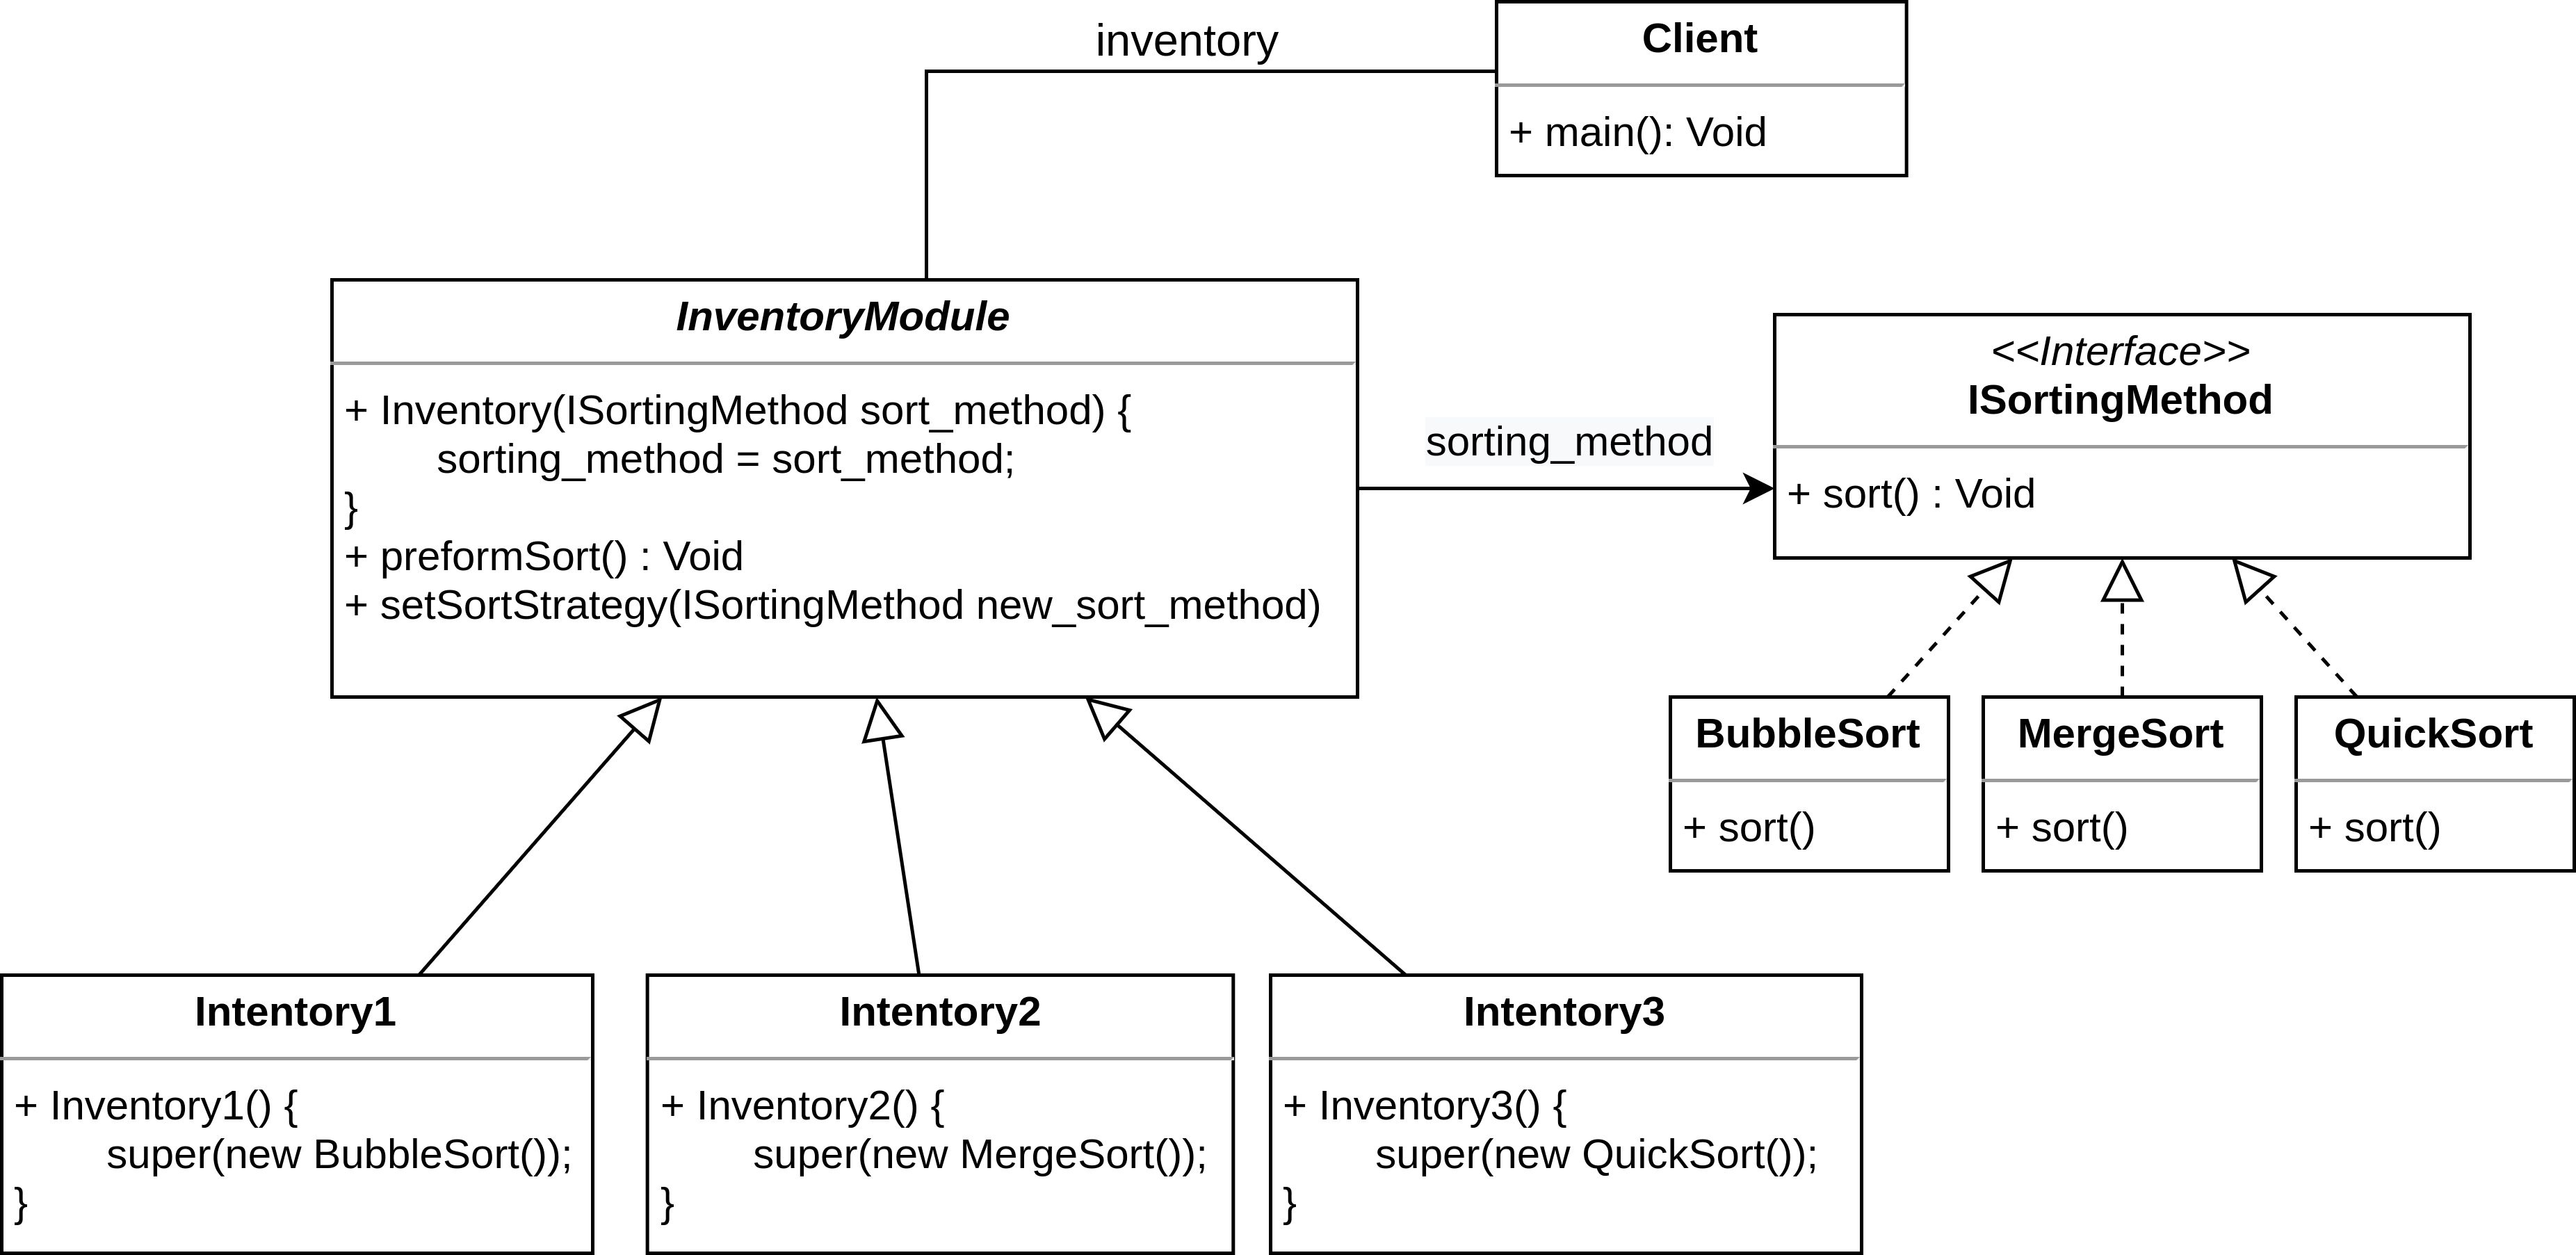
\includegraphics[width=\linewidth]{Class-Diagram.png}
\newpage
\section*{Java Code}


\subsection*{Client Class}
\begin{lstlisting}[language=Java]
// Client.java

import java.util.Scanner;

/**
 * Client class
 * 
 * - Main driver class for Homework 3
 *   - (i.e. has public static void main(String[] args))
 *   
 */
public class Client {

    // main method
    public static void main(String[] args) {

        // initialize local Inventory variable
        Inventory inventory = null;
        // initialize scanner, to read in user input from console
        Scanner console = new Scanner(System.in);
        // variable to store user input
        String user_selection = null;
        int user_int_selection = 0;

        /*
         * The following variables are used to by the application.
         * Either for output to the console or to maintain the 
         * running state.
         */

        Inventory[] inventory_arr = new Inventory[3];
        int current_inventory_index = 0;
        // string "constant", used for output to the user
        String dv = "----------------------------------------";
        // continue running application loop with true
        Boolean running = true;

        // output to user (via console)
        System.out.printf("%s\n%s\n%s\n", dv, "ESOF-322: Homework 3", dv);

        do {
            
            // Step 1: Select an Inventory Module
            // ------------------------------------------------------
            // - prompt the user to select an Inventory module.
            // - create the selected Inventory module and assign it
            // to the local variable 'inventory'.
            //

            // output to user
            System.out.printf("\n%s\n%s\n", "Step 1: Select an Inventory Module", dv);
            System.out.printf("%d - %s\n%d - %s\n%d - %s\n", 1, "Inventory1", 2, "Inventory2", 3, "Inventory3");

            // get user input from console (Scanner)
            System.out.print("('c' to exit) > ");
            user_selection = console.nextLine();

            // checked if user wants to exit
            if (user_selection.charAt(0) == 'c') { // user wants to exit
                running = false; // set running state to false
                continue;
            }

            try {
                user_int_selection = Integer.parseInt(user_selection);
            } catch (Exception e) {
                System.out.printf("%s: %s\n", "User Input Error", e.getMessage());
                continue;
            }

            current_inventory_index = user_int_selection - 1;

            if (inventory_arr[current_inventory_index] == null) {

                System.out.printf("\n%s\n%s\n", "New Inventory Module Created", dv);
                switch (user_int_selection) {
                    case 1:
                        inventory = new Inventory1();
                        break;
                    case 2:
                        inventory = new Inventory2();
                        break;
                    case 3:
                        inventory = new Inventory3();
                        break;
                    default:
                        System.out.println("\nInvalid input: " + user_selection);
                        continue;
                }
                inventory_arr[current_inventory_index] = inventory;
            } else {
                inventory = inventory_arr[current_inventory_index];
            }

            // Step 2: Perform default sorting method
            // ------------------------------------------------------
            //
            System.out.printf("\n%s\n%s\n", "Step 2: Perform (default) Sorting Method", dv);
            inventory.sort();

            // Step 3: Request User Selection
            // ------------------------------------------------------
            // Get a new sorting method from the user to dynamically
            // change the inventory's sorting behavior
            //
            
            System.out.printf("\n%s\n%s\n", "Step 3: Request User Selection (Sorting Method)", dv);
            System.out.printf("%d - %s\n%d - %s\n%d - %s\n", 1, "BubbleSort", 2, "MergeSort", 3, "QuickSort");

            // get user input from console (Scanner)
            System.out.print("('c' to exit) > ");
            user_selection = console.nextLine();

            // checked if user wants to exit
            if (user_selection.charAt(0) == 'c') { // user wants to exit
                running = false; // set running state to false
                continue;
            }

            // Step 4: Dynamically Change Sorting Method
            // ------------------------------------------------------
            // Set the inventory's sorting method dynamically
            //
            
            System.out.printf("\n%s\n%s", "Step 4: Dynamically Change Sorting Method", dv);
            switch (user_selection) {
                case "1": // Bubble Sort
                    inventory.setSortMethod(new BubbleSort()); // Change dynamically to BubbleSort
                    break;
                case "2": // Merge Sort
                    inventory.setSortMethod(new MergeSort()); // Change dynamically to MergeSort
                    break;
                case "3": // Quick Sort
                    inventory.setSortMethod(new QuickSort()); // Change dynamically to QuickSort
                    break;
                default: // Invalid selection from user input
                    System.out.println("\nInvalid input: " + user_selection);
                    continue;
            }

            // Step 5: Perform Sort
            // ------------------------------------------------------
            // Invoke the inventories sorting method behavior
            //
            
            System.out.printf("\n%s\n%s\n", "Step 5: Perform Sorting Method", dv);
            inventory.sort();

        } while (running); // END of application's loop
        
        console.close(); // Close the console (Scanner)
        
    } // END of Client::main method

} // END of Client class

\end{lstlisting}


\subsection*{ISortingMethod Interface}
\begin{lstlisting}[language=Java]
// ISortingMethod.java

/**
 * ISortingMethod (Interface)
 * 
 * This is the "behavior" interface for the sorting_method
 * 
 * Each of the unique sorting method type
 * must implement this interface, allowing the
 * Inventory Modules to sort a sorting behavior
 * as a composite value.
 * 
 * Each child class must provide:
 * - method "sort()"
 *
 */
public interface ISortingMethod {
    
    // all Sorting classes must implement their own sort function
    public void sort();
    
} // END of ISortingMethod class

\end{lstlisting}

\subsection*{BubbleSort Class}
\begin{lstlisting}[language=Java]
// BubbleSort.java

/**
 * BubbleSort class
 *
 * This is one of three possible sorting methods.
 * Each sorting type implements the ISortingMethod interface.
 * 
 */
public class BubbleSort implements ISortingMethod {

    // BubbleSorts implementation of the sort method
    public void sort() {
        System.out.println("--> BubbleSort::sort()\nPerforming BubbleSort...");
    } // END of sort() 
    
} // END of BubbleSort class

\end{lstlisting}

\subsection*{MergeSort Class}
\begin{lstlisting}[language=Java]
// MergeSort.java

/**
 * MergeSort class
 *
 * This is one of three possible sorting methods.
 * Each sorting type implements the ISortingMethod interface.
 * 
 */
public class MergeSort implements ISortingMethod {

    // MergeSorts implementation of the sort method
    public void sort() {
        System.out.println("--> MergeSort::sort()\nPerforming MergeSort...");
    } // END of sort() 
    
} // END of MergeSort class

\end{lstlisting}

\subsection*{QuickSort Class}
\begin{lstlisting}[language=Java]
// QuickSort.java

/**
 * QuickSort class
 *
 * This is one of three possible sorting methods.
 * Each sorting type implements the ISortingMethod interface.
 * 
 */
public class QuickSort implements ISortingMethod {

    // QuickSorts implementation of the sort method
    public void sort() {
        System.out.println("--> QuickSort::sort()\nPerforming Quicksort...");
    } // END of sort() 
    
} // END of QuickSort class

\end{lstlisting}

\subsection*{Inventory Class}
\begin{lstlisting}[language=Java]
// Inventory.java

/**
 * Inventory class (Abstract)
 * 
 * The individual Inventory Modules (Inventory1, Inventory2, and Inventory3)
 * extend this class to inherit common functionality.
 * 
 * Child classes define the "default" sorting method, or behavior,
 * in their constructors, which are passed to the parent constructor
 * via super(ISortingMethod)
 * 
 * The property 'sorting_method' or type ISortingMethod allows for
 * composition of a unique sorting method, and allows us to change
 * the behavior at runtime.
 *
 */
abstract public class Inventory {

    // The interface used by each unique sorting method type.
    public ISortingMethod sorting_method;
    
    
    // constructor
    public Inventory(ISortingMethod _sorting_method) {
        // set the default sorting method
        sorting_method = _sorting_method;
        // output statement to user
        System.out.println("Inventory Module: " + 
                this.toString().split("@")[0] +
                " \nDefault sorting method: " +
                sorting_method.toString().split("@")[0]);
    
    } // END of constructor
    
    
    /*
     * Sort()
     * 
     * Invokes the sorting method behavior
     * 
     */
    public void sort() {
        // output statement to user
        System.out.println("--> "+this.toString().split("@")[0] + "::sort()\nThe sorting method is: " + sorting_method.toString().split("@")[0]);
        sorting_method.sort();
    
    } // END of sort()

    
    /*
     * setSortMethod()
     * 
     * changes the default sorting method (dynamically) to the new one chosen by the user
     * 
     */
    public void setSortMethod(ISortingMethod method) {
        // dynamically set the sorting method (behavior)
        sorting_method = method;
        // cleanly prints out the new default sorting method to the user
        System.out.println("\n--> "+this.toString().split("@")[0]+"::setSortMethod(ISortingMethod method)\nDynamically set sorting method to: " + sorting_method.toString().split("@")[0]);
    
    } // END of setSortMethod()

} // END of Inventory class

\end{lstlisting}

\subsection*{Inventory1 Class}
\begin{lstlisting}[language=Java]
// Inventory1.java

/**
 * Inventory1 class
 * 
 * This inventory module extends the Inventory class.
 * 
 * The default sorting method is: Bubble Sort
 */
public class Inventory1 extends Inventory {

    // constructor
    public Inventory1() {
        // call parent constructor
        super(new BubbleSort()); // set default sorting method: BubbleSort
        
    } // END of constructor

} // END of Inventory1 class

\end{lstlisting}

\subsection*{Inventory2 Class}
\begin{lstlisting}[language=Java]
// Inventory2.java

/**
 * Inventory2 class
 * 
 * This inventory module extends the Inventory class.
 * 
 * The default sorting method is: Merge Sort
 */
public class Inventory2 extends Inventory {

    // constructor
    public Inventory2() {
        // call parent constructor
        super(new MergeSort()); // set default sorting method: MergeSort
    
    } // END of constructor

} // END of Inventory2 class

\end{lstlisting}

\subsection*{Inventory3 Class}
\begin{lstlisting}[language=Java]
// Inventory3.java

/**
 * Inventory3 class
 * 
 * This inventory module extends the Inventory class.
 * 
 * The default sorting method is: Quick Sort
 */
public class Inventory3 extends Inventory {

    public Inventory3() {
     // call parent constructor
        super(new QuickSort()); // set default sorting method: QuickSort
    
    } // END of constructor

} // END of Inventory3 class

\end{lstlisting}

\newpage
\section*{Sequence Diagram}
\end{document}
